\chapter{EmberVLM: Efficient Edge Vision-Language Model}
\label{cha:embervlm}

This chapter presents EmberVLM, the primary architectural contribution of this thesis. EmberVLM is a 164M total parameter (40M trainable) tiny VLM purpose-built for reliable mission-critical inference under strict edge-deployment constraints. It builds directly on the design principles established in BitMar (Chapter~\ref{cha:bitmar}), scaling to a more capable backbone while introducing two novel modules: the Episodic Memory Module and the Visual Absence (VA) Refiner.

\section{Overview and Design Philosophy}
\label{sec:embervlm_overview}

Figure~\ref{fig:embervlm_arch} illustrates the complete EmberVLM architecture. EmberVLM is guided by three design principles:

\begin{enumerate}
    \item \textbf{Compositional efficiency}: separate frozen pretrained representations (DINOv2-Small for visual perception, SmolLM-135M for linguistic priors) from a compact trainable core (40M parameters). This preserves the general capabilities of large pretraining while keeping training cost and carbon emissions minimal.
    \item \textbf{Memory-augmented reliability}: treat episodic memory not as a static knowledge base but as a dynamically loadable, deployment-time cache that provides contextual biases drawn from prior field experience. Memory breaks the traditional latency--accuracy tradeoff by providing near-zero-cost retrieval from a compact on-device matrix.
    \item \textbf{Mechanistic hallucination control}: instead of suppressing hallucinations through additional supervision or retraining, identify and penalize visually ungrounded tokens at inference time by monitoring the model's own internal neuron-level activation patterns.
\end{enumerate}

\begin{sidewaysfigure}[p]
    \centering
    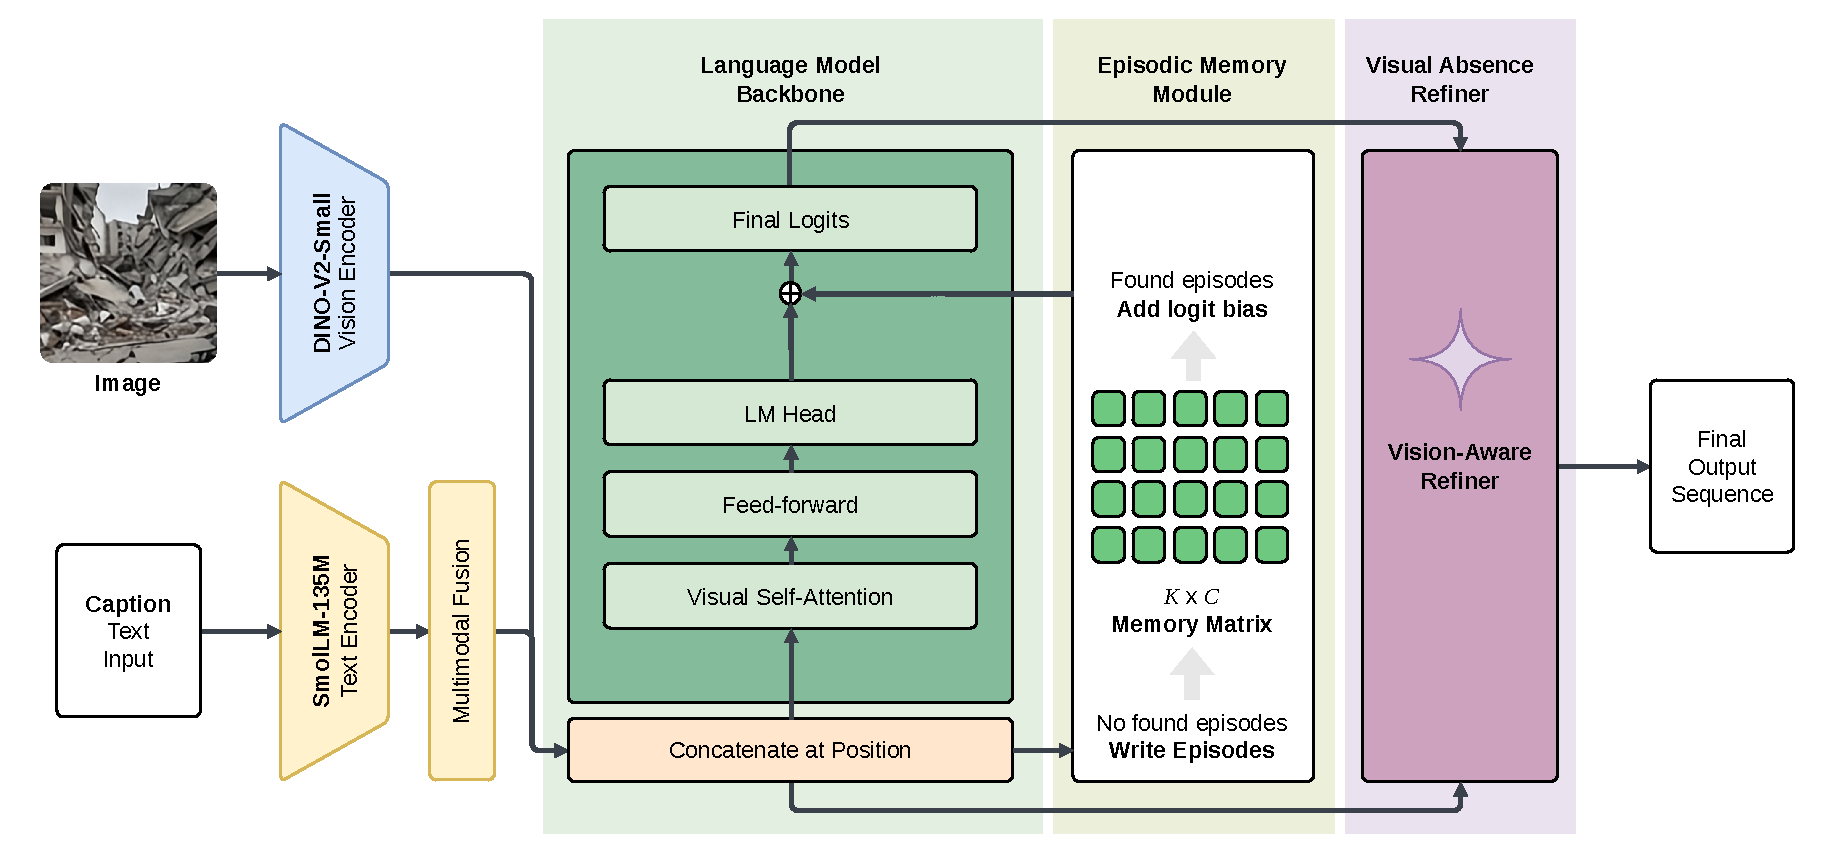
\includegraphics[width=\textheight]{../EmberVLM/paper-template-Latest/figures/main_diagram.pdf}
    \caption{\textbf{EmberVLM architecture overview.} The system integrates a frozen DINOv2-Small vision encoder, a SmolLM-135M language backbone, a Stable Gated Fusion module, an Episodic Memory Module, and the Visual Absence (VA) Refiner. Solid arrows denote forward-pass data flow; the memory matrix is outside the gradient graph and is updated algebraically at deployment time.}
    \label{fig:embervlm_arch}
\end{sidewaysfigure}

\section{Base Multimodal Pipeline}
\label{sec:embervlm_base}

\subsection{Vision Encoder}
EmberVLM employs DINOv2-Small~\cite{oquab2024dinov2} as the frozen visual perception module (21.1M parameters). The encoder aggressively compresses an input image $X_v$ into a minimal sequence of $N_v{=}8$ visual tokens with feature dimension $d_{\text{vis}}{=}384$. DINOv2-Small's self-supervised training provides robust visual features without task-specific supervision, and freezing it throughout training preserves general visual priors while contributing zero parameters to the trainable budget.

\subsection{Language Backbone}
SmolLM-135M~\cite{allal2024smollm} serves as both the text encoder and the language modeling backbone (135M parameters). SmolLM-135M is frozen in Stages 1, 3, and 4, and fully unfrozen end-to-end in Stage 2 (Multimodal Instruction Tuning). This staged approach allows the model to first learn cross-modal alignment while preserving linguistic priors, then adapt the full backbone to complex multimodal instruction following.

\subsection{Parameter Breakdown}

Figure~\ref{fig:embervlm_params_dist} illustrates the distribution of parameters across components. Of the 164M total parameters, only 40M (24.4\%) are updated during training; the remaining 75.6\% are frozen pretrained representations that contribute visual and linguistic priors at zero training cost.

\begin{figure}[!htb]
    \centering
    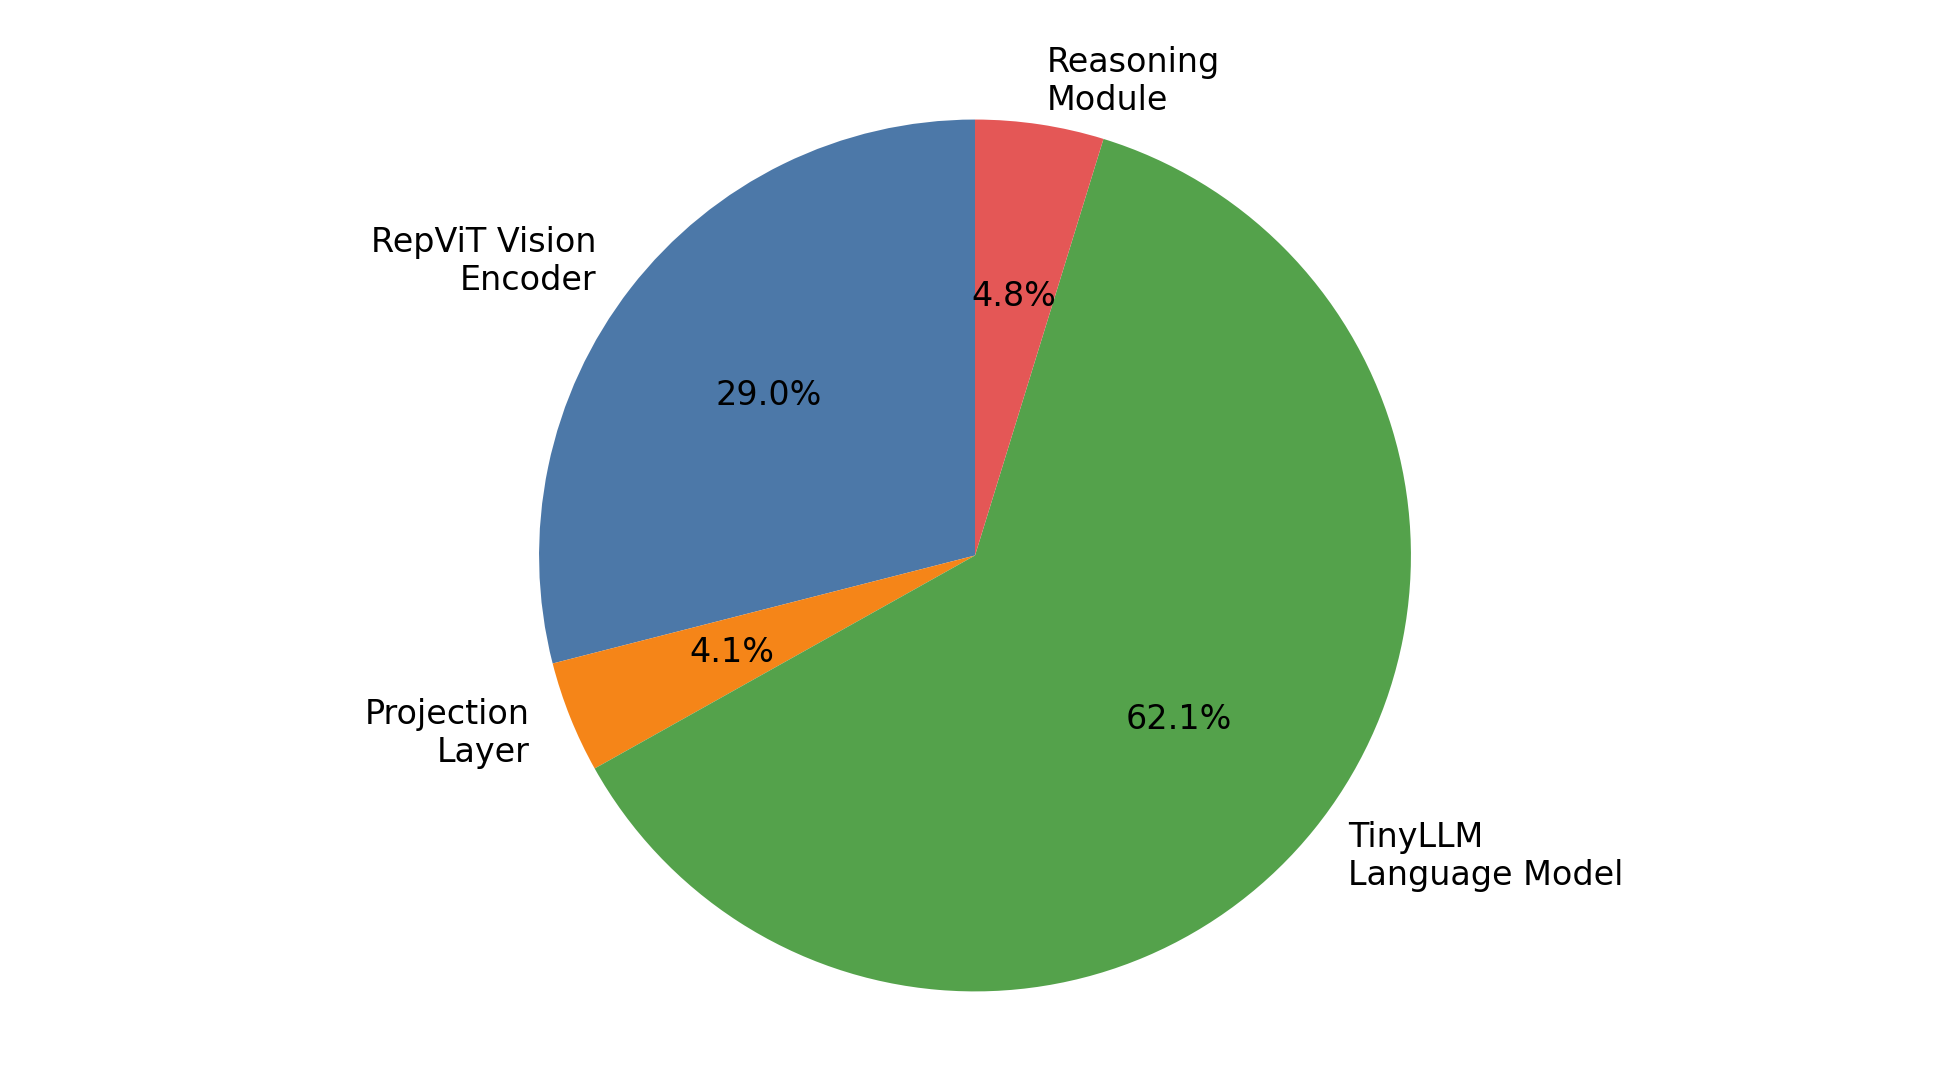
\includegraphics[width=0.65\linewidth]{../EmberVLM/paper-template-Latest/figures/embervlm_param_distribution.png}
    \caption{\textbf{EmberVLM parameter distribution.} DINOv2-Small (21.1M) and the frozen layers of SmolLM-135M account for the majority of total parameters and are never updated. The 40M trainable parameters are concentrated in the Fusion Module, bottleneck adapter, and Reasoning Head.}
    \label{fig:embervlm_params_dist}
\end{figure}

\begin{table}[htbp]
\centering
\caption{\textbf{EmberVLM parameter breakdown.} Total: 164M parameters, 40M trainable.}
\label{tab:embervlm_params}
\resizebox{\textwidth}{!}{%
\begin{tabular}{llcc}
\toprule
\textbf{Component} & \textbf{Params (M)} & \textbf{Trainable} & \textbf{Frozen Stages} \\
\midrule
DINOv2-Small (vision encoder) & 21.1 & --- & All stages \\
SmolLM-135M (text enc. + backbone) & 135.0 & Partial & 1, 3, 4 \\
Fusion Module (cross-attn + gate) & 7.27 & \checkmark & None \\
Bottleneck adapter & 0.06 & \checkmark & None \\
Reasoning \& Action Head & 0.57 & \checkmark & 1, 2 \\
\midrule
\textbf{Total} & \textbf{164.0} & \textbf{40M} & --- \\
\bottomrule
\end{tabular}%
}
\end{table}

\begin{table}[htbp]
\centering
\caption{\textbf{EmberVLM architectural specification.} Component-level summary of the 164M-parameter system, including encoder, backbone, memory, and VA Refiner configuration.}
\label{tab:embervlm_arch_spec}
\begin{tabular}{ll}
\toprule
\textbf{Component} & \textbf{Specification} \\
\midrule
Vision encoder & DINOv2-Small (21.1M, frozen) \\
Visual tokens $N_v$ & 8 \\
Visual feature dim $d_{\text{vis}}$ & 384 \\
Language backbone & SmolLM-135M (135M) \\
Language feature dim $d_{\text{lang}}$ & 576 \\
Bottleneck adapter dim & 48 \\
Vision gate initialization $\alpha$ & 2.5 \\
Episodic memory slots $K$ & 512 \\
Episodic memory dim $C$ & 576 \\
Memory size (fp32) & $\approx$1.2 MB \\
VA Refiner hook layers & 10--14 (SmolLM-135M FFN) \\
VA Refiner neuron count & 128 (top-$k$ per layer) \\
VA Refiner $\lambda$ & 0.5 \\
Visual threshold $p_{\text{VA}}$ & 0.6 \\
Non-visual threshold $p_{\text{VA}}$ & 0.8 \\
Latent CoT temperature $\tau$ & 0.07 \\
\bottomrule
\end{tabular}
\end{table}

\section{Stable Gated Fusion}
\label{sec:embervlm_fusion}

Raw visual tokens from DINOv2-Small (dimension 384) are projected into the language backbone's token embedding space ($d_{\text{lang}}{=}384$) via a parameter-efficient bottleneck adapter ($d_{\text{bottleneck}}{=}48$). A learnable vision gate scalar $\alpha$ (initialized to 2.5) dynamically scales the adapted visual influence:
\begin{equation}
    V_{\text{fused}} = \sigma(\alpha) \cdot \mathrm{LayerNorm}(V_{\text{adapt}})
    \label{eq:embervlm_gate}
\end{equation}
where $\sigma$ denotes the sigmoid activation. At initialization, $\sigma(2.5) \approx 0.92$, so visual influence starts near-full and becomes learnable rather than fixed. This gate allows the model to calibrate how much visual influence to apply during alignment learning, preventing early-stage visual features from overwhelming linguistic priors.

The gated visual tokens are interleaved with textual embeddings to form the joint context sequence processed by the language backbone.

\section{Task-Specific Adaptation: Top-$K$ Robot Selection Head}
\label{sec:embervlm_head}

While EmberVLM supports standard autoregressive generation, autoregressive decoding is inefficient and error-prone for mission-critical tactical deployment. For the primary robot selection task, the standard language modeling head is bypassed. Instead, final hidden states from the language backbone are mean-pooled to produce a dense incident representation $\mathbf{h}_{\text{pool}}$. A \textit{Reasoning and Action Head} MLP maps $\mathbf{h}_{\text{pool}}$ to a probability distribution over the robot fleet (Drone, Underwater Robot, Humanoid, Wheeled, Legged):
\begin{equation}
    \mathbf{p}_{\text{robot}} = \mathrm{softmax}\!\left(\mathrm{MLP}(\mathbf{h}_{\text{pool}})\right)
\end{equation}
This framing decouples general scene comprehension from tactical execution. Avoiding autoregressive decoding eliminates the token-by-token latency overhead, keeping total trainable parameters strictly under 40M.

\section{Episodic Memory Module}
\label{sec:embervlm_memory}

\subsection{Overview and Distinction from BitMar}
EmberVLM's episodic memory differs fundamentally from BitMar's gradient-trained memory. BitMar's memory matrix is updated via backpropagation and is static at deployment. EmberVLM's memory has three key properties:
\begin{itemize}
    \item \textbf{Outside the gradient graph}: the memory matrix is not differentiated through, as confirmed in the supplementary material.
    \item \textbf{Pre-populated offline}: populated from the training split during a READ\_ONLY pre-population phase before evaluation.
    \item \textbf{Updatable online at deployment}: in ONLINE\_UPDATE mode, new embeddings are written to memory during inference without weight updates, enabling adaptation to novel scenarios.
\end{itemize}

\subsection{Memory Matrix Specification}
The memory matrix $\mathbf{M} \in \mathbb{R}^{K \times C}$ has $K{=}512$ slots and $C{=}576$ feature dimensions, alongside an associated covariance matrix. Physical size: $512 \times 576 \times 4$ bytes $\approx$ 1.2~MB (fp32). The dimension $C{=}576$ matches the SmolLM-135M token embedding dimension, allowing direct residual injection of retrieved memory into the generation process without additional projection overhead.

\subsection{Scope Detector}
Before engaging memory retrieval, the incoming multimodal embedding $\mathbf{z}$ is evaluated by a lightweight Scope Detector: a 2-layer MLP binary classifier outputting $p(\text{in-scope})$. If $p < 0.5$, the query is deemed out-of-scope and the model defaults to parametric generation without memory. If $p \geq 0.5$, the fast memory retrieval path activates.

The scope detector serves as a gating mechanism that prevents irrelevant historical episodes from contaminating queries about novel or out-of-distribution scenes. Without scope detection, the memory module would apply retrieved context to every query, potentially degrading performance on genuinely novel scenarios.

\subsection{Memory Addressing and Retrieval}
When in-scope, normalized addressing weights $w_k$ over all $K$ memory slots are computed via Gaussian distance-based addressing:
\begin{equation}
    w_k = \frac{\exp\!\left(-\dfrac{\|\mathbf{z} - \mathbf{M}_k\|^2}{2\alpha\nu\tau}\right)}{\displaystyle\sum_{j=1}^{K} \exp\!\left(-\dfrac{\|\mathbf{z} - \mathbf{M}_j\|^2}{2\alpha\nu\tau}\right)}
    \label{eq:embervlm_mem_address}
\end{equation}
where $\alpha$, $\nu$, $\tau$ represent the update strength, variance, and temperature scaling factors, respectively. The retrieved memory readout $\mathbf{z}_m = \sum_k w_k \mathbf{M}_k$ is passed through the language model's unembedding head and added residually to the raw predictive logits, organically biasing generation toward historically successful resolutions.

This mechanism is more sophisticated than BitMar's content-based addressing in that it includes explicit variance ($\nu$) and temperature ($\tau$) parameters that control the sharpness of retrieval, allowing fine-tuned control over how broadly or narrowly the model draws from past experience.

\subsection{Novelty Detection and Dynamic Writes}
\label{sec:memory_novelty}
The novelty of an incoming embedding $\mathbf{z}$ is defined as:
\begin{equation}
    \sigma(\mathbf{z} \mid \mathbf{M}) = \min_k \|\mathbf{z} - \mathbf{M}_k\|^2
\end{equation}
If this minimum-distance novelty score exceeds a predefined threshold, the incident is classified as a fundamentally new experience. The system executes a single-shot recursive algebraic update using a linear solve over the residual difference between the new embedding and the current memory readout, updating both $\mathbf{M}$ and the covariance matrix.

When the memory reaches $K$-slot capacity, a hybrid Least Recently Used and Least Frequently Used (LRU-LFU) eviction policy selects the slot to overwrite. LRU alone risks discarding slots encoding critical rare morphologies (e.g., Underwater Robot, which appears in only 13 of the 103 validation samples); LFU alone risks retaining stale commonly-accessed but no-longer-relevant episodes. The hybrid policy balances recency and importance.

\subsection{Stage 5 Knowledge Consolidation}
During an optional Stage 5 consolidation phase, the frozen memory matrix acts as a teacher: an MSE alignment loss distills explicitly retrieved knowledge directly into the model's parametric weights. This ensures that frequently accessed experiences become ingrained in base model weights, freeing memory slots for new encounters. Stage 5 is not applied in any of the main paper evaluation results; it is a deployment-phase enhancement.

\subsection{Complete Memory Inference Procedure}

Algorithm~\ref{alg:embervlm_memory} summarizes the full episodic memory procedure executed at each inference step, unifying scope detection, Gaussian retrieval, novelty-triggered writes, and LRU-LFU eviction into a single coherent procedure.

\begin{algorithm}[htbp]
\small
\caption{EmberVLM episodic memory: scope detection, retrieval, novelty write, and LRU-LFU eviction.}
\label{alg:embervlm_memory}
\begin{algorithmic}[1]
\Require Query $\mathbf{z} \in \mathbb{R}^C$, memory $\mathbf{M} \in \mathbb{R}^{K \times C}$, covariance $\boldsymbol{\Sigma}$,
\Statex \hspace{\algorithmicindent} novelty threshold $\theta$, LRU-LFU balance $\gamma$,
\Statex \hspace{\algorithmicindent} mode $\in \{\texttt{OFF},\; \texttt{READ\_ONLY},\; \texttt{ONLINE\_UPDATE}\}$
\Ensure Residual logit bias $\Delta\mathbf{l}$, updated $\mathbf{M}$
\If{mode $= \texttt{OFF}$}
    \State \Return $\Delta\mathbf{l} \leftarrow \mathbf{0}$ \Comment{memory bypassed}
\EndIf
\State $p_{\text{scope}} \leftarrow \text{ScopeDetector}(\mathbf{z})$ \Comment{2-layer MLP binary classifier}
\If{$p_{\text{scope}} < 0.5$}
    \State \Return $\Delta\mathbf{l} \leftarrow \mathbf{0}$ \Comment{out-of-scope: use parametric generation}
\EndIf
\State $w_k \leftarrow \exp\!\bigl(-\|\mathbf{z} - \mathbf{M}_k\|^2 / (2\alpha\nu\tau)\bigr)$ for $k=1,\ldots,K$
\State $\mathbf{w} \leftarrow \mathbf{w} / \textstyle\sum_k w_k$ \Comment{Gaussian addressing weights}
\State $\mathbf{z}_m \leftarrow \textstyle\sum_k w_k \mathbf{M}_k$ \Comment{weighted memory readout}
\State $\Delta\mathbf{l} \leftarrow \text{UnembeddingHead}(\mathbf{z}_m)$ \Comment{residual logit bias}
\If{mode $= \texttt{ONLINE\_UPDATE}$}
    \State $\sigma_{\text{nov}} \leftarrow \min_k \|\mathbf{z} - \mathbf{M}_k\|^2$ \Comment{novelty score}
    \If{$\sigma_{\text{nov}} > \theta$} \Comment{novel: write to memory}
        \If{empty slot $k^*$ available}
            \State $k^* \leftarrow$ index of first empty slot
        \Else \Comment{LRU-LFU hybrid eviction}
            \State $k^* \leftarrow \arg\max_k\bigl[\gamma \cdot \text{age}(k) - (1{-}\gamma) \cdot \text{freq}(k)\bigr]$
        \EndIf
        \State $\mathbf{M}_{k^*} \leftarrow \mathbf{z}$; update $\boldsymbol{\Sigma}$; reset age/freq for $k^*$
    \EndIf
\EndIf
\State \Return $\Delta\mathbf{l}$, $\mathbf{M}$
\end{algorithmic}
\end{algorithm}

\subsection{Memory Operating Modes}

Three memory modes are available at deployment time, as specified in Table~\ref{tab:memory_modes_spec}.

\begin{table}[htbp]
\centering
\caption{\textbf{EmberVLM episodic memory operating modes.} The three runtime modes control whether the memory matrix is read, written, or inactive during inference.}
\label{tab:memory_modes_spec}
\begin{tabularx}{\textwidth}{lX}
\toprule
\textbf{Mode} & \textbf{Description} \\
\midrule
OFF & Memory matrix is zeroed; scope detector is bypassed; model operates in parametric generation mode for all queries. \\
\midrule
READ\_ONLY & Memory pre-populated from training split embeddings before evaluation. No writes occur during evaluation, eliminating label leakage risk. Used for all primary evaluation results. \\
\midrule
ONLINE\_UPDATE & Memory is both read and written during evaluation. For in-scope queries: retrieve context, evaluate novelty, and if novel execute a single-shot algebraic update with hybrid LRU-LFU eviction at $K$-slot capacity. Simulates live edge deployment. \\
\bottomrule
\end{tabularx}
\end{table}

\section{Visual Absence (VA) Refiner}
\label{sec:embervlm_refiner}

\subsection{Motivation}
EmberVLM without the VA Refiner achieves a 29\% hallucination rate on the POPE Adversarial split. For robot selection, where hallucinating a ``Wheeled Robot'' when the scene shows a ``Drone'' leads to wrong deployment, this rate is unacceptable. Three constraints eliminate most prior mitigation methods: (1) no retraining, (2) no extra forward passes, (3) no labeled grounding data.

\subsection{Dual-View Consistency Pathway}
At each generation step, the model computes logits twice: once with visual context ($L_{\text{vis}}$) and once with visual tokens ablated ($L_{\text{ablated}}$). The logit-based visual absence score:
\begin{equation}
    s_{\text{logit}} = 1.0 - \tanh\!\left(\left|L_{\text{vis}} - L_{\text{ablated}}\right|\right)
    \label{eq:va_logit}
\end{equation}
A high $s_{\text{logit}}$ indicates the token is equally likely with or without the image, signaling weak visual grounding. The tanh normalizes the discrepancy to $[0, 1]$ and provides soft rather than binary thresholding.

\subsection{Neuron-Level Activation Pathway}
A feature extractor hooks into the FFN modules across mid-decoder layers 10 through 14 of SmolLM-135M, capturing the top-128 neuron activations per layer. These activations are processed by a lightweight Continuous MLP classifier to generate a neuron-based visual absence probability $p_{\text{neuron}}$.

The classifier is trained offline on SmolLM-135M FFN activations from training-split samples only. Labels are generated automatically by comparing per-token probabilities with and without visual token ablation; no human annotation is required. The classifier is fit on a frozen backbone snapshot from Stage 2.

The mechanistic rationale is illustrated in Figure~\ref{fig:embervlm_neuron}: for hallucinated tokens, mid-decoder neuron activation patterns remain symmetric regardless of whether visual input is present, indicating generation from language priors alone. For correctly grounded tokens, activation patterns change substantially when the image is removed, confirming structural dependence on actual visual content. The VA Refiner exploits this discrepancy as a hallucination signal.

\begin{figure}[!htb]
    \centering
    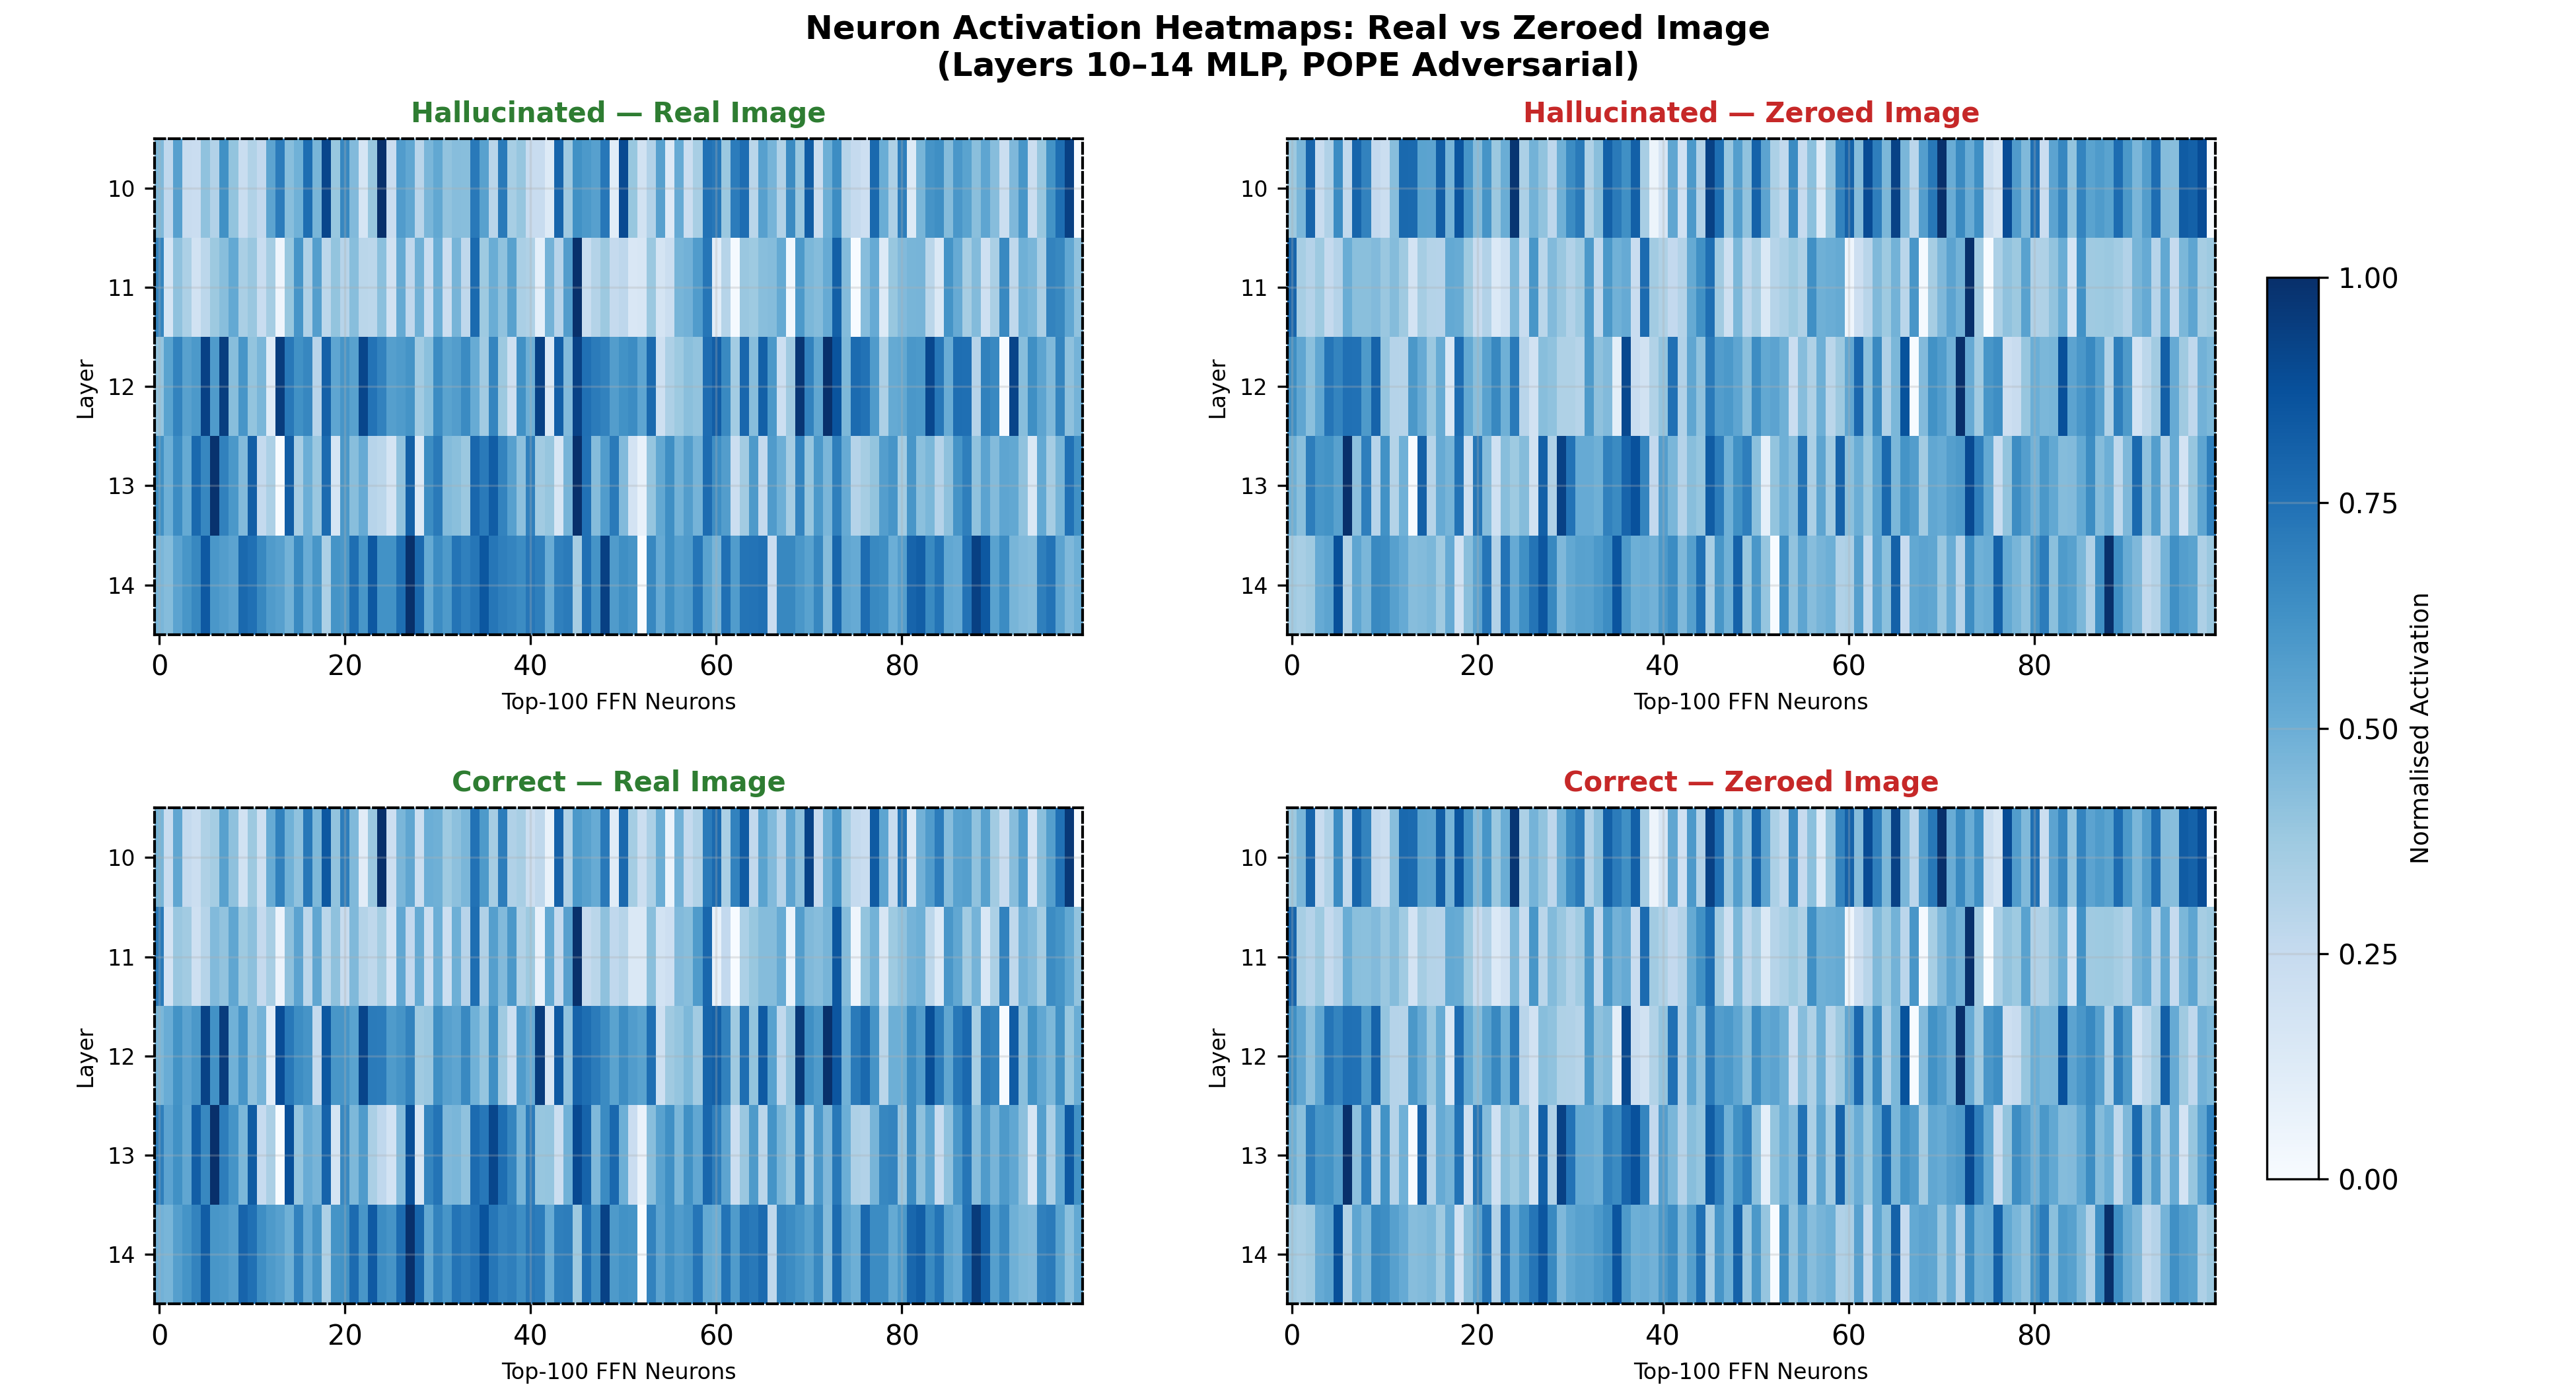
\includegraphics[width=\textwidth]{../EmberVLM/paper-template-Latest/figures/va_ablation_neuron_heatmap.png}
    \caption{\textbf{Neuron activation heatmaps.} \textbf{Top:} For hallucinated cases, activation patterns are nearly identical with and without the image, indicating generation from language priors. \textbf{Bottom:} For correctly grounded cases, activations change substantially when the image is removed, demonstrating reliance on actual visual content.}
    \label{fig:embervlm_neuron}
\end{figure}

\subsection{Combined Visual Absence Score}
The final visual absence probability for a given token combines both pathways:
\begin{equation}
    p_{\text{VA}} = \lambda \cdot p_{\text{neuron}} + (1-\lambda) \cdot s_{\text{logit}}
    \label{eq:va_combined}
\end{equation}
where $\lambda{=}0.5$ balances internal representation confidence against output distribution consistency.

\subsection{Type-Aware Intervention}
Using a heuristic dictionary of visually sensitive keywords (objects, colors, spatial relations), sensitive tokens face a strict hallucination threshold ($p_{\text{VA}} \geq 0.6$), while non-visual tokens face a looser boundary ($p_{\text{VA}} \geq 0.8$). Tokens exceeding their respective thresholds receive a severe logit penalty, forcing the model to select a more visually grounded alternative.

\subsection{Temporal Burst Detection}
Since hallucinations often occur in cascading clusters, the VA Refiner maintains a sliding-window temporal memory of recent $p_{\text{VA}}$ scores. If the moving average exceeds a predefined burst threshold, the refiner escalates from soft penalty to hard block (token logit $= -\infty$) and dampens the output distribution to break generative momentum.

\subsection{Mission Uncertainty Calibration}
After a full sequence is generated, the system aggregates $p_{\text{VA}}$ scores for all visually sensitive tokens. If the average absence score falls within a critical boundary, a system-level uncertainty flag is raised. Rather than prepending conversational caveats to the output, this flag signals the downstream autonomous controller that the current visual--tactical alignment is low-confidence, allowing the system to request a secondary camera angle or defer to human operator judgment. This transforms the VA Refiner from a pure text-generation mechanism into a systems-level reliability signal.

\subsection{Complete VA Refiner Inference Procedure}

Algorithm~\ref{alg:va_refiner} formalizes the full per-token intervention logic, integrating dual-view scoring, type-aware thresholding, and temporal burst detection into the decoding loop.

\begin{algorithm}[htbp]
\small
\caption{Visual Absence (VA) Refiner: per-token hallucination detection and logit intervention.}
\label{alg:va_refiner}
\begin{algorithmic}[1]
\Require Logits $L_{\text{vis}}$ (with image), $L_{\text{ablated}}$ (image ablated),
\Statex \hspace{\algorithmicindent} mid-decoder FFN activations $\mathbf{A}_{10:14}$,
\Statex \hspace{\algorithmicindent} thresholds $p^{\text{vis}}_{\text{VA}}{=}0.6$, $p^{\text{nonvis}}_{\text{VA}}{=}0.8$,
\Statex \hspace{\algorithmicindent} burst window $B$, burst threshold $\beta$, combination weight $\lambda{=}0.5$
\Ensure Adjusted logits $L_{\text{out}}$, system uncertainty flag
\State $s_{\text{logit}} \leftarrow 1.0 - \tanh(|L_{\text{vis}} - L_{\text{ablated}}|)$ \hfill\Comment{Eq.~\ref{eq:va_logit}}
\State $p_{\text{neuron}} \leftarrow \text{ContinuousMLP}(\text{top-}128(\mathbf{A}_{10:14}))$
\State $p_{\text{VA}} \leftarrow \lambda \cdot p_{\text{neuron}} + (1-\lambda) \cdot s_{\text{logit}}$ \hfill\Comment{Eq.~\ref{eq:va_combined}}
\State Append $p_{\text{VA}}$ to sliding window $W_{\text{burst}}$ of length $B$
\If{$\mathrm{mean}(W_{\text{burst}}) > \beta$} \Comment{hallucination burst}
    \State $L_{\text{out}} \leftarrow -\infty$; dampen output distribution
    \State \textbf{raise} system uncertainty flag; \Return $L_{\text{out}}$
\EndIf
\State sensitive $\leftarrow$ IsVisuallySensitive(current token, keyword dictionary)
\State threshold $\leftarrow$ $p^{\text{vis}}_{\text{VA}}$ if sensitive else $p^{\text{nonvis}}_{\text{VA}}$
\If{$p_{\text{VA}} \geq$ threshold}
    \State $L_{\text{out}} \leftarrow L_{\text{vis}} - \text{SeverePenalty}(\text{top-}k\text{ ungrounded candidates})$
\Else
    \State $L_{\text{out}} \leftarrow L_{\text{vis}}$ \Comment{no intervention needed}
\EndIf
\State \Return $L_{\text{out}}$
\end{algorithmic}
\end{algorithm}

\section{Four-Stage Training Curriculum}
\label{sec:embervlm_training_curriculum}

EmberVLM is trained through four supervised stages, each targeting a distinct capability, as illustrated in Figure~\ref{fig:embervlm_stages}. Training datasets are summarized in Table~\ref{tab:embervlm_datasets}, and hyperparameters in Table~\ref{tab:embervlm_hyperparams}.

\begin{figure}[!htb]
    \centering
    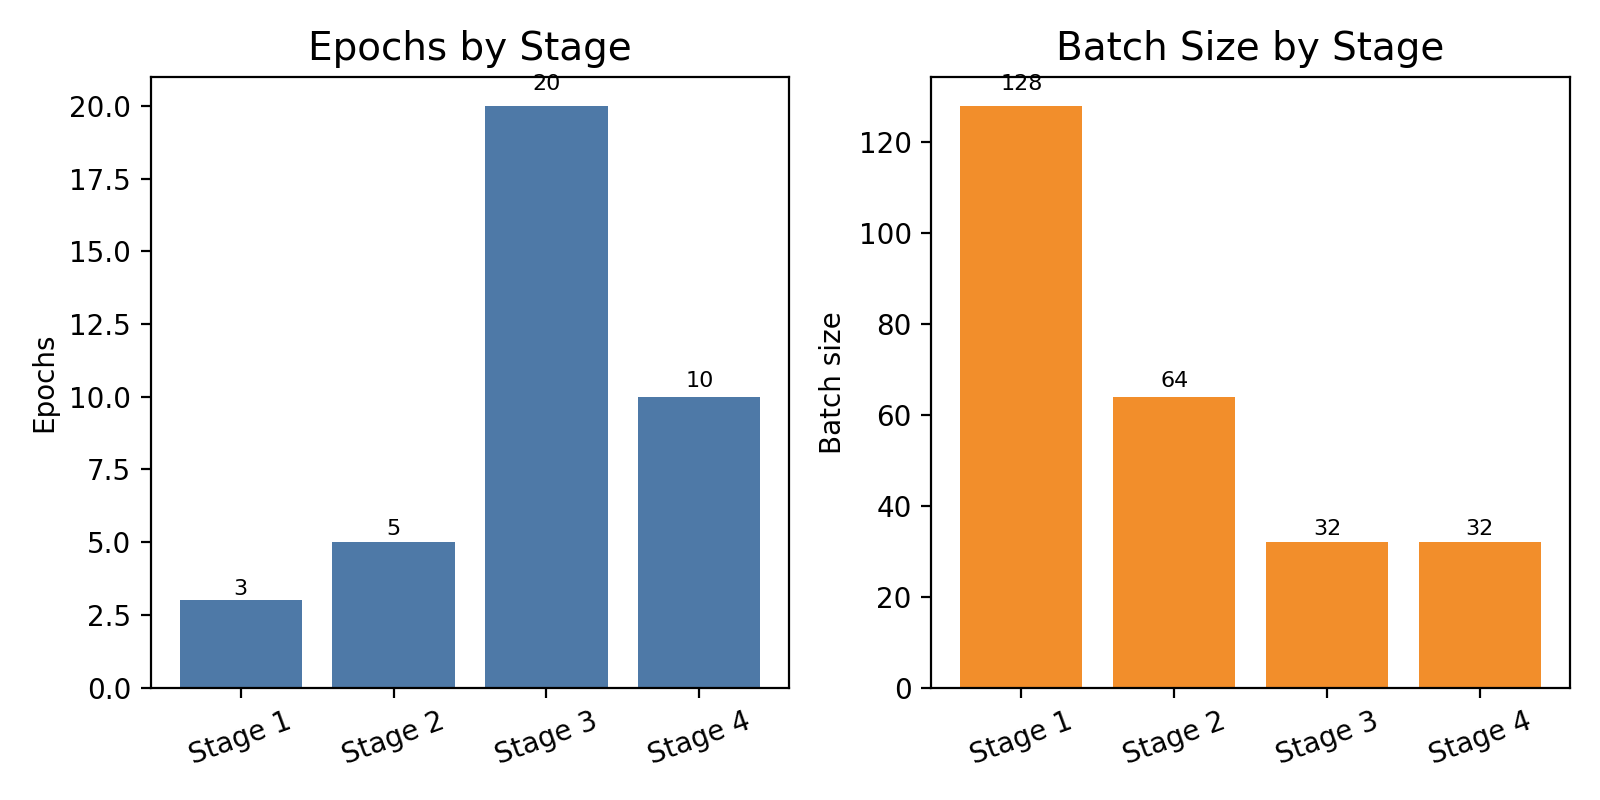
\includegraphics[width=\textwidth]{../EmberVLM/paper-template-Latest/figures/fig_training_stages.png}
    \caption{\textbf{EmberVLM four-stage training curriculum.} Stage~1 freezes both backbones and trains only the Fusion Module for visual-language alignment. Stage~2 unfreezes the language backbone for instruction tuning. Stage~3 re-freezes the backbone and trains the Reasoning Head for robot fleet selection. Stage~4 trains the Reasoning Head via InfoNCE contrastive loss to align internal step-embeddings with procedurally generated chain-of-thought rationales.}
    \label{fig:embervlm_stages}
\end{figure}

\begin{table}[htbp]
\centering
\caption{\textbf{EmberVLM training datasets across all stages.}}
\label{tab:embervlm_datasets}
\begin{tabular}{llc}
\toprule
\textbf{Stage} & \textbf{Dataset} & \textbf{Epochs} \\
\midrule
\multirow{8}{*}{1: Alignment} & CC3M~\cite{sharma2018cc3m} & 10 \\
 & RefCOCO~\cite{yu2016refcoco} & 10 \\
 & VQA v2~\cite{VQA} & 10 \\
 & COCO Annotations~\cite{lin2014coco} & 10 \\
 & LLaVA~\cite{liu2023llava} & 10 \\
 & OK-VQA~\cite{marino2019okvqa} & 10 \\
 & A-OKVQA~\cite{schwenk2022aokvqa} & 10 \\
 & GQA~\cite{hudson2019gqa} & 10 \\
\midrule
2: Instruction Tuning & LLaVA Instruct 150K & 15 \\
\midrule
3: Task Adaptation & Robot Selection & 20 \\
\midrule
4: Latent CoT & Robot Selection (CoT) & 10 \\
\bottomrule
\end{tabular}
\end{table}

\begin{figure}[!htb]
    \centering
    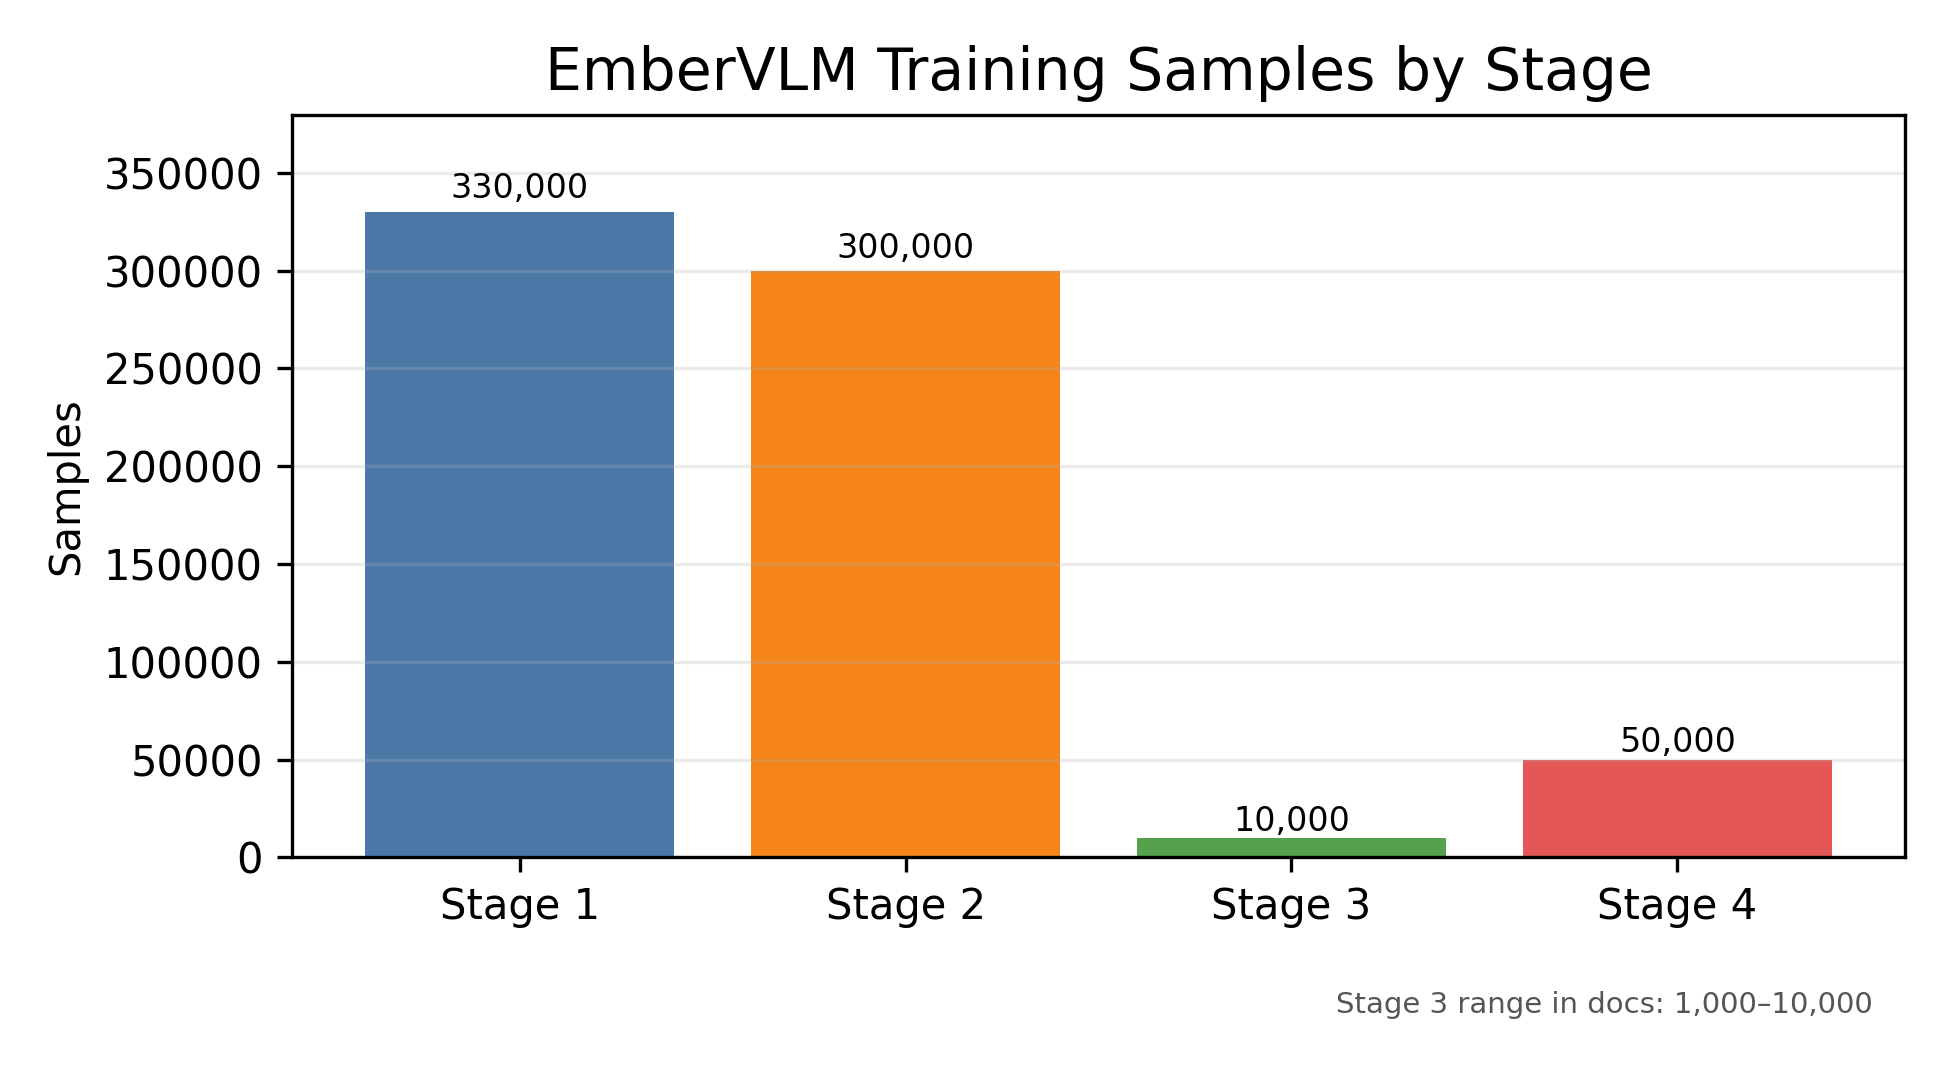
\includegraphics[width=\textwidth]{../EmberVLM/paper-template-Latest/figures/embervlm_stage_samples.png}
    \caption{\textbf{Representative training samples across stages.} Stage~1 alignment samples pair images with short captions. Stage~2 instruction tuning samples involve multi-turn visual dialogue. Stages~3--4 use structured robot-selection prompts with multi-label annotations and programmatic chain-of-thought rationales.}
    \label{fig:embervlm_stage_samples}
\end{figure}

\begin{table}[htbp]
\centering
\caption{\textbf{EmberVLM training hyperparameters by stage.}}
\label{tab:embervlm_hyperparams}
\resizebox{\textwidth}{!}{%
\begin{tabular}{lcccc}
\toprule
\textbf{Stage} & \textbf{LR} & \textbf{Eff. Batch} & \textbf{Max Seq.} & \textbf{Unfrozen Components} \\
\midrule
1: Alignment & $2\times10^{-4}$ & 256 & 512 & Fusion Module only \\
2: Instruction & $2\times10^{-4}$ & 256 & 512 & Fusion + Language Backbone \\
3: Task Adapt. & $1\times10^{-4}$ & 128 & 256 & Reasoning \& Action Head \\
4: Latent CoT & $1\times10^{-4}$ & 128 & 256 & Reasoning Head \\
\midrule
\multicolumn{5}{l}{\textit{All stages: AdamW ($\lambda_{\text{wd}}{=}10^{-2}$), cosine LR with 5\% warmup, bf16 mixed precision, 2$\times$A100.}} \\
\bottomrule
\end{tabular}%
}
\end{table}

\subsection{Stage 1: Visual-Language Alignment}
Vision and language backbones remain frozen; only the Fusion Module is actively trained. The model learns to map raw DINOv2 visual features into meaningful linguistic token space by predicting captions and answering standard visual queries across eight diverse datasets. This stage establishes the multimodal grounding capability without modifying the pretrained language or vision representations.

Figure~\ref{fig:stage1_heatmap} visualizes how text-to-patch attention evolves across training checkpoints during Stage 1. At the start of training (top row), attention is diffuse and unstructured. By mid-training (middle row), the model begins concentrating attention on semantically relevant regions consistent with the caption. By the end of Stage 1 (bottom row), attention is sharply localized to the salient scene elements described in the caption, confirming that the Fusion Module has learned to ground linguistic concepts in specific image patches.

\begin{figure}[!htb]
    \centering
    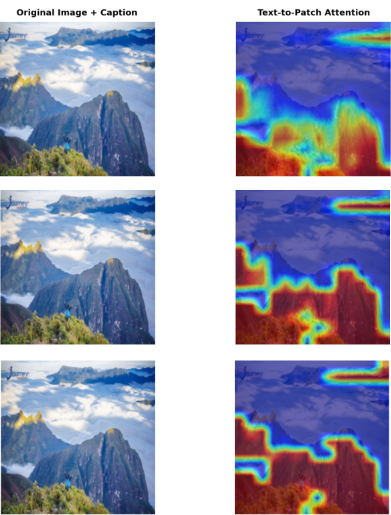
\includegraphics[width=0.85\linewidth]{heatmap_stage1.png}
    \caption{\textbf{Text-to-patch attention progression during Stage 1 alignment training.} Each row shows a training checkpoint (early, mid, late). The left column shows the input image with its associated caption; the right column shows the corresponding text-to-patch attention heatmap. Warm colors (red/yellow) indicate high attention weight on image patches. As training progresses, diffuse initial attention concentrates onto the semantically relevant regions of the scene, demonstrating the Fusion Module's acquisition of cross-modal visual grounding.}
    \label{fig:stage1_heatmap}
\end{figure}

\subsection{Stage 2: Multimodal Instruction Tuning}
The vision encoder remains frozen, but both the Fusion Module and the Language Backbone are fully unfrozen and fine-tuned end-to-end on LLaVA Instruct 150K. This enables the model to interpret nuanced human instructions and engage in multi-turn visual dialogue grounded in image content. Unfreezing the backbone in Stage 2 is the primary source of adaptable capacity in EmberVLM's training.

\subsection{Stage 3: Robot Fleet Selection}
The standard autoregressive head is bypassed, and the Reasoning and Action Head is unfrozen and trained with cross-entropy loss for Top-$K$ robot classification on the Robot Selection dataset. The backbone is re-frozen in this stage to prevent catastrophic forgetting of the instruction-tuning knowledge acquired in Stage 2.

\subsection{Stage 4: Latent Chain-of-Thought Integration}
Rather than predicting explicit CoT text tokens (which would add autoregressive latency at inference time), the Reasoning Head is trained to align its internal step-embeddings with procedurally generated Chain-of-Thought rationales using an InfoNCE contrastive loss ($\tau{=}0.07$):
\begin{equation}
    \mathcal{L}_{\text{CoT}} = -\log \frac{\exp(\mathrm{sim}(\mathbf{h}_{\text{reason}}, \mathbf{r}_{\text{CoT}})/\tau)}{\sum_{j}\exp(\mathrm{sim}(\mathbf{h}_{\text{reason}}, \mathbf{r}_j)/\tau)}
\end{equation}
Rationales are generated programmatically via a fixed rule-based template, requiring no external teacher model or human annotation:
\begin{verbatim}
"Scene analysis: [scene_description].
 Environmental condition: [condition].
 Required capability: [capability].
 Recommended robot type: [type].
 Reasoning: [rule-based justification]."
\end{verbatim}
Templates are instantiated from scene labels, environmental tags, and robot capability requirements from the dataset annotation. By training the head to align its \emph{internal embeddings} with CoT rationales rather than generating them token-by-token, EmberVLM gains deductive transparency without any inference-time latency penalty.

\section{Dynamic Tiered Memory Management}
\label{sec:embervlm_tiered_memory}

Figure~\ref{fig:embervlm_edge} shows the edge deployment scenario targeted by EmberVLM. Rather than pinning the entire 164M-parameter architecture in active compute memory, EmberVLM employs a dynamic tiered memory management strategy.

\begin{figure}[!htb]
    \centering
    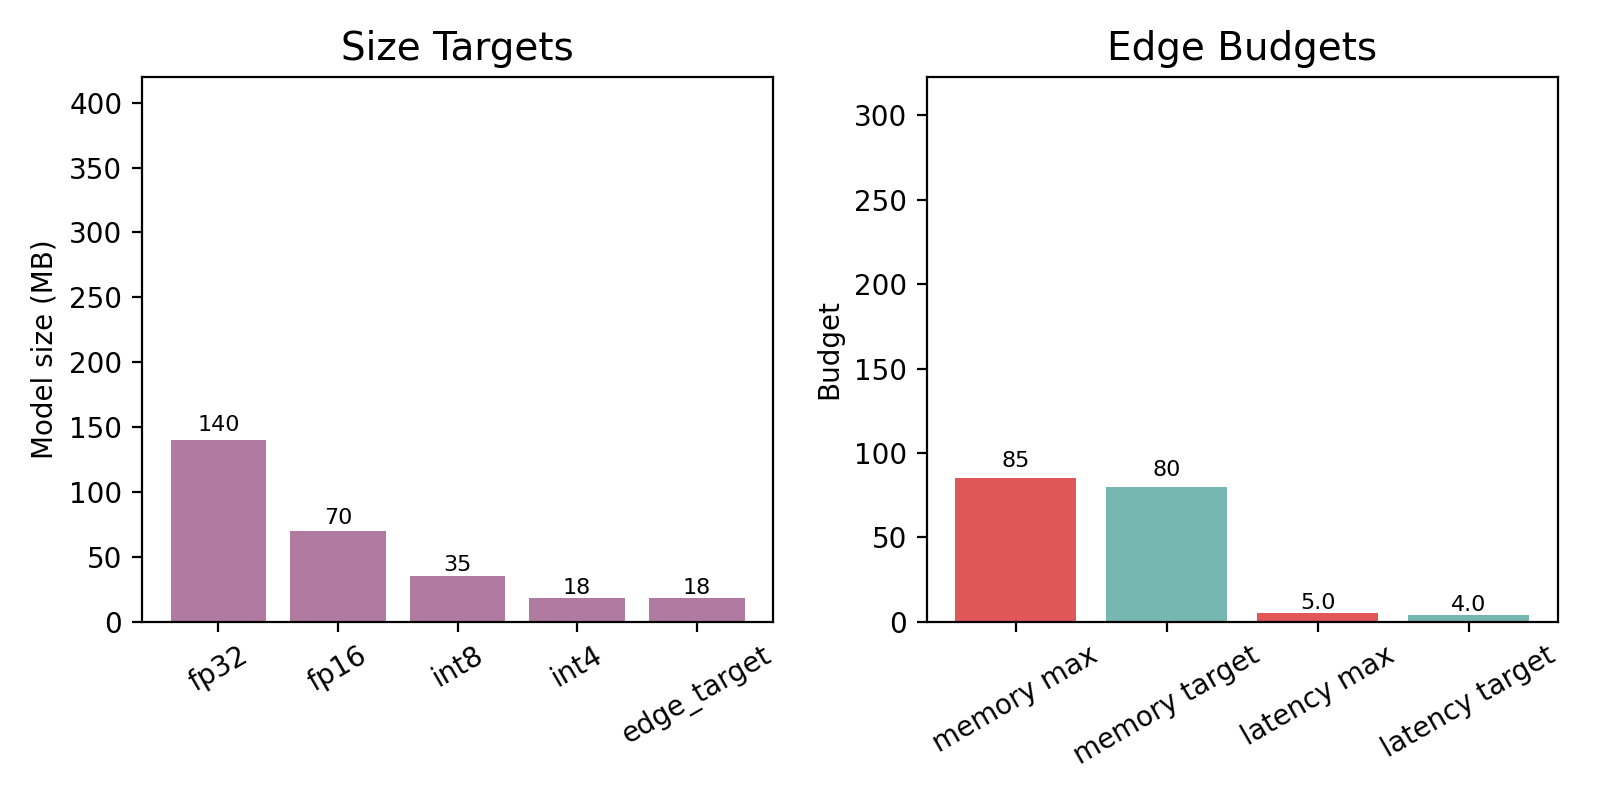
\includegraphics[width=0.9\linewidth]{../EmberVLM/paper-template-Latest/figures/fig_edge_targets.png}
    \caption{\textbf{Target edge deployment environments.} EmberVLM is designed for CPU-only hardware platforms such as the AMD Ryzen 3 4100 (3.80~GHz, 32~GB RAM, no discrete GPU), representative of resource-constrained field units used in emergency response, autonomous robotics, and remote sensing applications.}
    \label{fig:embervlm_edge}
\end{figure} The lightweight scope detector and the $512 \times 576$ memory matrix are permanently pinned to the primary compute device (total: $\sim$1.2~MB + scope detector parameters). For historically seen instances where the scope detector registers high confidence, the system directly retrieves contextual biases from memory without loading the full parametric model.

On AMD Ryzen 3 4100 (3.80 GHz, 32 GB RAM, no GPU), the full EmberVLM stack (Model + VA Refiner + Memory) operates at 5.22~ms per sample, consuming $<$800~MB RAM. For comparison, InternVL3-1B requires a discrete GPU with 1{,}978~MB VRAM and achieves only 1{,}566~ms per sample on the same hardware, making it categorically unsuitable for the target deployment regardless of its benchmark scores.

\section{Carbon Footprint Analysis}
\label{sec:embervlm_carbon}

\begin{table}[htbp]
\centering
\caption{\textbf{Training carbon emissions (CodeCarbon-measured).} All values are measured, not estimated. Training on 2$\times$A100 GPUs.}
\label{tab:embervlm_emissions}
\resizebox{\textwidth}{!}{%
\begin{tabular}{lrrc}
\toprule
\textbf{Stage} & \textbf{Duration} & \textbf{Emissions (kg CO$_2$eq)} & \textbf{\% of Total} \\
\midrule
Stage 1: Alignment     & 50 h (5 epochs)  & 16.6513 & 65.6\% \\
Stage 2: Instruction   & 40 h (13 epochs) & 8.6545  & 34.1\% \\
Stage 3: Robot Sel.    & $\approx$20 min  & 0.0046  & 0.02\% \\
Stage 4: Reasoning     & $\approx$10 min  & 0.0062  & 0.02\% \\
\midrule
\textbf{Total} & $\approx$90 h & \textbf{25.3166} & 100\% \\
\bottomrule
\end{tabular}%
}
\end{table}

Total measured training emissions across all stages are 25.3~kg CO$_2$eq, approximately equivalent to driving 100~km in an average gasoline car, and more than 21{,}000$\times$ less than GPT-3's estimated 552 tonnes CO$_2$eq~\cite{patterson2021carbon}. By constraining trainable parameters to 40M and completing all alignment and instruction tuning within approximately 90 hours on dual A100s, EmberVLM demonstrates that mission-critical capable multimodal AI can be trained sustainably. This positions low-carbon training not merely as a byproduct of efficiency but as a first-class design objective.

Carbon emissions were measured using CodeCarbon~\cite{codecarbon} integrated directly into the training loop. Measurements record actual power consumption of the 2$\times$A100 GPU cluster (hardware power draw via NVML), CPU, and memory, multiplied by the carbon intensity of the Taiwan electricity grid (approximately 0.509~kg~CO$_2$eq/kWh during the measurement period). All figures in Table~\ref{tab:embervlm_emissions} are \emph{measured}, not estimated from FLOPs or parameter counts.
